\documentclass{article}
\usepackage[utf8]{inputenc}

% Basic packages
	\usepackage{amssymb}
	\usepackage{amsmath}
	\usepackage{graphicx}
	\usepackage[english]{babel}
	\usepackage{natbib}

% Relevant packages
	\usepackage{bm}
	\usepackage{bbm}
	\usepackage{geometry}
	\usepackage{enumitem}
	\usepackage{listings}

% Document settings
	\geometry{a4paper,margin=15mm}

	\setlist[itemize]{nolistsep,noitemsep}
		
	\setlength{\parindent}{0pt}
	\setlength{\parskip}{1.5em}
	\renewcommand{\baselinestretch}{1.2}

	\setlength{\abovedisplayskip}{1.2em}
	\setlength{\belowdisplayskip}{1.2em}
	\renewcommand{\arraystretch}{1.2}

\begin{document}
	\section{pohybová rovnice diskretizované soustavy}
	``\emph{Zapište pohybovou rovnici diskretizované soustavy (analogicky rovnici rovnováhy ze statiky ve tvaru $\bm{K}\bm{U} = \bm{F}$. Vysvětlete význam jednotlivých členů.}''

	\begin{equation}
		\bm{M}\bm{\ddot{\delta}} + \bm{C}\bm{\dot{\delta}} + \bm{K}\bm{\delta} - \bm{F} = \bm{0}
	\end{equation}
	\begin{itemize}
		\item [$\bm{\delta}$] - vektor uzlových posuvů
		\item [$\bm{M}$] - matice hmotnosti
		\item [$\bm{C}$] - matice tlumení
		\item [$\bm{K}$] - matice tuhosti
		\item [$\bm{F}$] - vektor vnějších sil
	\end{itemize}

	\section{diferenční operátor}
	\emph{``Vysvětlete pojem \textbf{diferenční operátor} (diferenční schéma). Jako příklad navrhněte diferenční schéma pro diferenciální operátory $\frac{d\bm{U}}{dt},\frac{d^2\bm{U}}{dt^2}$.''}

	Diferenční operátor je takový operátor, kterým dokážeme aproximovat derivaci funkce v daném bodě pomocí hodnot funkce v jeho okolí (moje definice).
	
	Vychází z taylorova rozvoje
	\begin{equation}
		\bm{U}(t_0+\Delta t) \approx \bm{U}(t_0) + \frac{d\bm{U}(t_0)}{dt} \Delta t + \frac{d^2\bm{U}(t_0)}{2\,dt^2} \Delta t^2 + \dots
	\end{equation}
	
	\subsection{Dopředná diference prvního řádu}
	
	První derivaci lze aproximovat jako
	\begin{equation}
		\frac{d\bm{U}(t_0)}{dt} \approx \frac{\bm{U}(t_0+\Delta t) - \bm{U}(t_0)}{\Delta t}
	\end{equation}
	s výslednou diferencí
	\begin{equation}
		\frac{d\bm{U}_{t_0}}{dt} = \frac{\bm{U}_{t_0+\Delta t} - \bm{U}_{t_0}}{\Delta t}
	\end{equation}
	
	\subsection{Centrální diference druhého řádu}

	Centrální diferenci druhého řádu získáme dosazením centrální diference prvního řádu
	\begin{equation}
		\frac{d\bm{U}(t_0)}{dt} \approx \frac{\bm{U}(t_0+\Delta t) - \bm{U}(t_0-\Delta t)}{2\Delta t}
	\end{equation}
	za první derivaci.
	% \begin{equation}
	% 	\bm{U}(t_0+\Delta t) \approx \bm{U}(t_0) + \frac{\bm{U}(t_0+\Delta t) - \bm{U}(t_0-\Delta t)}{2} + \frac{d^2\bm{U}(t_0)}{2\,dt^2} \Delta t^2 + \dots
	% \end{equation}
	Úpravou získáme approximaci druhé derivace
	\begin{equation}
		\frac{d^2\bm{U}(t_0)}{dt^2}
		\approx
		\frac{ \bm{U}(t_0+\Delta t) - 2\bm{U}(t_0) + \bm{U}(t_0-\Delta t) }{\Delta t^2}
	\end{equation}
	ze které plyne diferenční schéma
	\begin{equation}
		\frac{d^2\bm{U}_{t_0}}{dt^2}
		=
		\frac{\bm{U}_{t_0+\Delta t} - 2\bm{U}_{t_0} + \bm{U}_{t_0-\Delta t}}{\Delta t^2}
	\end{equation}

	\section{Konzistence matice hmotnosti}
	\emph{``Vysvětlete pojmy konzistentní a nekonzistentní matice hmotnosti a vztah k explicitnímu integračnímu schématu. Jakou výhodu přináší užití nekonzistentní matice a za jakou cenu?''}

	Konzistentní matice hmotnosti vzniká sestavením z matic hmotnosti elementů ve tvaru $\bm{M}^e = \int_{(V_e)} \bm{N}^T \rho \, dV$ (konzistentním s energetickým přístupem), které obsahují i mimo diagonální prvky. Pak se rovnice netlumeného systému řeší rozkladem matice $\bm{M}$ do diagonálního tvaru.

	Existuje přístup ke konstrukci matice hmotnosti, který rozdělí hmotu elementu do uzlů (aproximace). Pak má matice hmotnosti systému (stejně jako jednotlivé matice elementů) pouze diagonální členy a názýváme ji nekonzistentní.

	\section{Modální transformace}
	\emph{``Definujte operátor (matici) modální transformace $\Phi$, popište jeho vlastnosti a naznačte transformaci rovnice (*) do modálních souřadnic.''}

	Je-li matice $\Phi$ řešením problému vlastních čísel
	\begin{equation}
		\bm{K}\bm{\Phi} = \bm{\Omega}^2 \bm{M} \bm{\Phi}
	\end{equation}
	kde $\bm{\phi}_i$ jsou vlastní vektory a $\omega_i$ vlastní frekvence tvořící matice $\bm{\Phi}$ a $\bm{\Omega}$  
	\begin{equation}
		\bm{\Phi} = \begin{bmatrix} \bm{\phi}_i & \dots & \bm{\phi}_N \end{bmatrix}
		\,,\;
		\bm{\Omega}^2 = \operatorname{diag}(\omega_i^2)
		\;,\quad 
		i \in \langle 1,N \rangle
	\end{equation}
	platí
	\begin{equation}
		\bm{\Phi}^T\bm{M}\bm{\Phi} = \bm{1}
		\;,\quad 
		\bm{\Phi}^T\bm{K}\bm{\Phi} = \bm{\Omega}^2
	\end{equation}

	Soustavu pohybovných rovnic systému s proporčním tlumením
	\begin{equation}
		\bm{M}\bm{\ddot{\delta}} + \bm{C}\bm{\dot{\delta}} + \bm{K}\bm{\delta} = \bm{F}
	\end{equation}
	lze zavedením modální souřadnice $\bm{q} = \bm{\Phi}\bm{\delta}$ a vynásobením transponovanou maticí modální transformace $\bm{\Phi}^T$ zleva, převést do tvaru
	\begin{equation}
		\bm{\ddot{q}} + \bm{\Gamma}\bm{\dot{q}} + \bm{\Omega}^2 \bm{q} = \bm{\Phi}^T \bm{F}
		\;,\quad 
		\bm{\Gamma} = \operatorname{diag}(2\,\omega_i\xi_i) \;,\quad i \in \langle 1,N \rangle
	\end{equation}
	kde $\xi_i$ jsou poměrné útlumy.

	Soustava se pak rozpadá na rovnice ve tvaru
	\begin{equation}
		\ddot{q}_i + 2\,\omega_i\xi_i \dot{q} + \omega_i^2 q = f_i
		\;,\quad 
		f_i = \bm{\phi}_i \cdot \bm{F}
		\;,\quad 
		i \in \langle 1,N \rangle
	\end{equation}

	\section{Deformační gradient}
	\emph{``Zapište vztah mezi elementární úsečkou v referenční konfiguraci (popsanou vektorem $d\bm{X}$) a toutéž úsečkou (popsanou vektorem $d\bm{x}$) v konfiguraci aktuální. Popište vlastnosti operátoru, který tento vztah zprostředkuje.''}
	
	\begin{equation}
		d\bm{x} = \bm{F} \, d\bm{X}
	\end{equation}
	přičemž $\bm{F}$ je regulární tzn. $\det(\bm{F}) > 0$ a dále platí
	\begin{equation}
	\bm{F} = \bm{1} + \bm{Z}
	\;,\quad 
	\bm{Z} = \frac{\partial \bm{u}}{\partial \bm{X}}
	\end{equation}
	také lze rozložit jako
	\begin{equation}
	\bm{F} = \bm{R}(\bm{X},t)\,\bm{U}(\bm{X},t)
	\end{equation}
	kde $\bm{R}$ je tenzor rotace (ortonormální) a $\bm{U}$ tenzor ryzí deformace (symetrický).
	
	\subsection{Greenův-Langrangeův tenzor deformace}
	Pomocí deformačního gradientu lze definovat Greenův-Langrangeův tenzor deformace
	\begin{equation}
	\bm{e} = \frac{1}{2}(\bm{F}^T\bm{F} - \bm{1}) = \frac{1}{2}(\bm{U}^T\bm{U} - \bm{1})
	\end{equation}

	\section{Newton–Raphsonovo schéma}
	\emph{``Popište princip Newton–Raphsonova iteračního schématu v přírůstkové metodě. Využijte grafické znázornění pro jeden stupeň volnosti a pro soustavu s mnoha stupni volnosti naznačte vývojový diagram.''}
	\begin{enumerate}
		\item $\bm{u} = \bm{u}_0$
		\item $\bm{F}^I = \bm{K}_T(\bm{u})\,\bm{u}$
		\item $\bm{F}^N = \bm{F}^E - \bm{F}^I$
		\item $\|\bm{F}^N\| < \varepsilon$ \textbf{?} return \textbf{:} nothing
		\item $\Delta \bm{u} = \bm{K}_T(\bm{u})^{-1} \bm{F}^N$
		\item $\bm{u} = \bm{u} + \Delta \bm{u}$
		\item zpět na 2.
	\end{enumerate}
	\begin{figure}[h!]
		\centering
		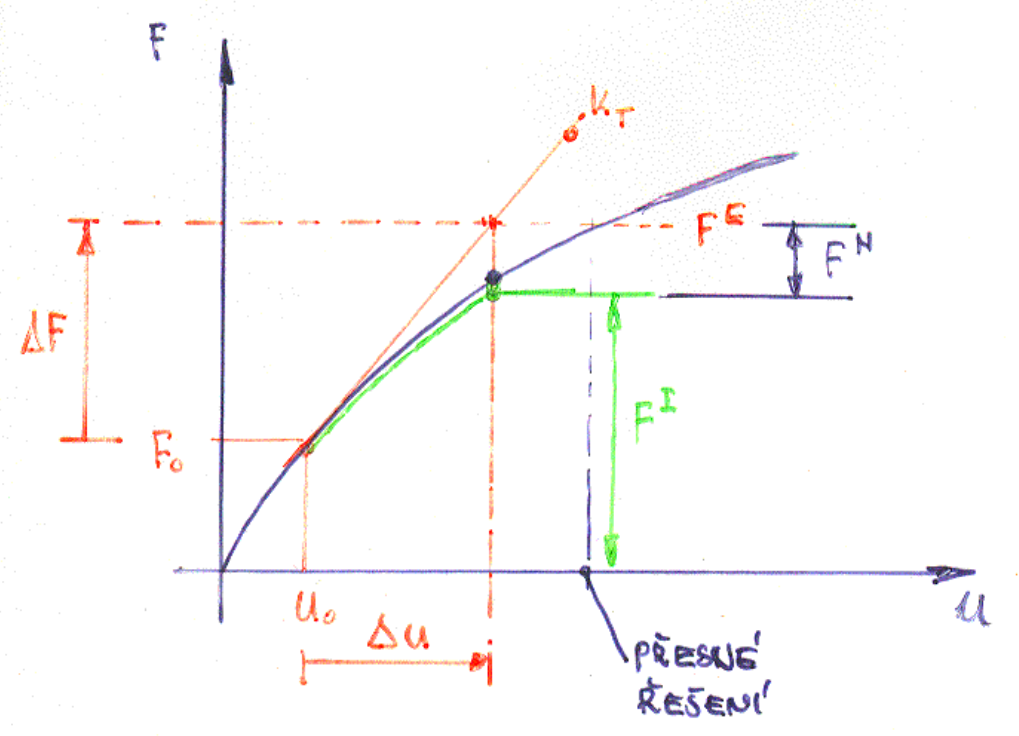
\includegraphics[width=.5\linewidth]{figs/NR1.png}
	\end{figure}
	\begin{figure}[h!]
		\centering
		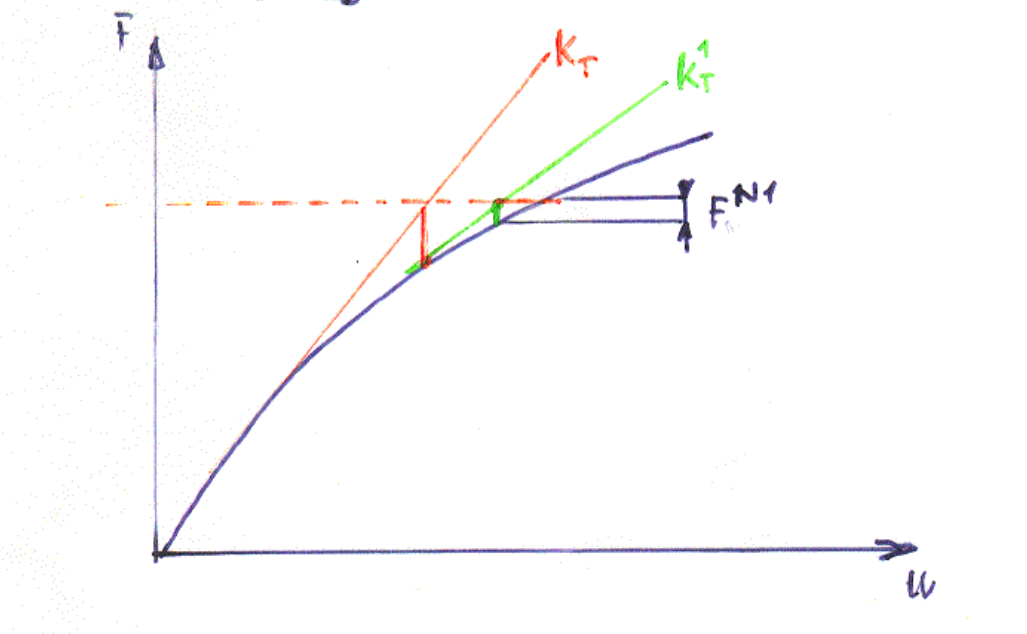
\includegraphics[width=.5\linewidth]{figs/NR2.png}
	\end{figure}

	\section{Nelineární model}

	\section{Zpevňování}
	\emph{``Vysvětlete pojmy kinematické a izotropní zpevnění.''}

	Trojosá napjatost je obecně popsána bodem v 6D hyper-prostoru. Vzhledem k symetrii tenzoru napětí lze množinu všech možných stavů napětí zakreslit jako oblast v prostoru hlavních napětí.

	Průmět oblasti do deviatorické roviny budeme nazývat plochou plasticity, přičemž na její hranici se budou nacházet průměty napětí elasto-plastické deformace, zatímco uvnitř stavy elastické deformace.

	Při zpevňování bude docházet k plastickému tečení, v jehož průběhu se mění plocha plasticity. Pro ideální plastický materiál se tvar plochy nemění (nejsem si jistý), pouze se zvětšuje (\textbf{isotropní zpevňování}) nebo posouvá (\textbf{kinematické zpevňování}).
	\begin{figure}[h!]
		\centering
		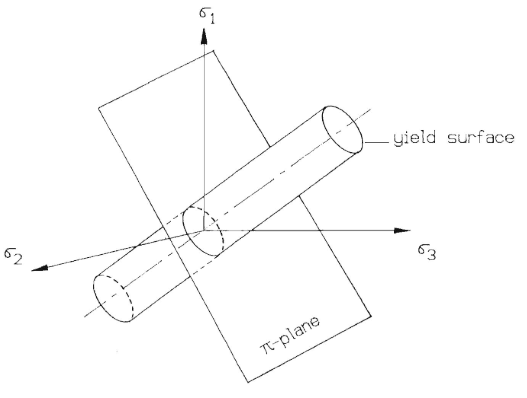
\includegraphics[width=.5\linewidth]{figs/PlochaPlasticity.png}
	\end{figure}
	\begin{figure}[h!]
		\centering
		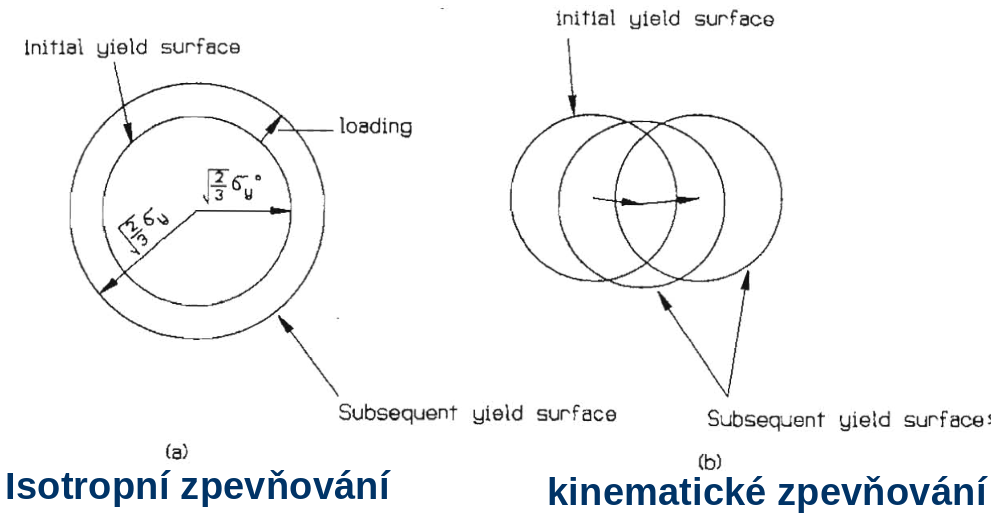
\includegraphics[width=.5\linewidth]{figs/Zpevnovani.png}
	\end{figure}

	\section{Tečná matice tuhosti a stabilita systému}
	\emph{``Jaký je vztah mezi tečnou maticí tuhosti a stabilitou systému?''}

	\section{Status kontaktního páru}
	\emph{``Vysvětlete pojem status kontaktního páru (za kontaktní pár považujte pro jednoduchost dvojici uzlů potenciálně svázaných kontaktní vazbovou rovnicí) a formulujte podmínky pro změnu statusu.''}

	Kontaktní podmínku páru uzlů lze zapsat jako
	\begin{equation}
		(\bm{u}_2 - \bm{u}_1 ) \cdot \bm{n} = \delta
	\end{equation}
	Status kontaktního páru lze určit z hodnoty $\delta$
	\begin{equation}
		\text{status} = \left\{
		    \begin{array}{ll}
		    	\delta < 0 : \text{``spojeno''} \\
		    	\delta > 0 : \text{``rozpojeno''}
		    \end{array}
		    \right.
	\end{equation}
	nebo pomocí reakce
	\begin{equation}
		\text{status} = \left\{
		    \begin{array}{ll}
		    	\bm{R}_{12} \cdot \bm{n} < 0 : \text{``spojeno''} \\
		    	\bm{R}_{12} \cdot \bm{n} > 0 : \text{``rozpojeno''}
		    \end{array}
		    \right.
	\end{equation}
	Pokud je okamžitý status ``spojeno'', provádíme kontrolu pomocí reakce a v statusu ``rozpojeno'' přes hodnotu $\delta$.
	\begin{figure}[h!]
		\centering
		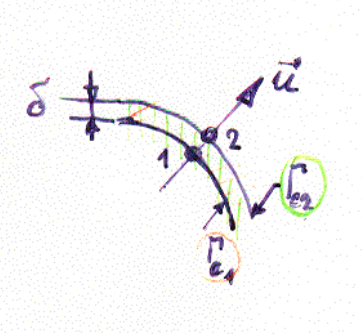
\includegraphics[width=.5\linewidth]{figs/KontaktniPar.png}
	\end{figure}

	\section{Iterační schéma kontaktní úlohy}
	\emph{``Naznačte iterační schéma kontaktní úlohy (za kontaktní pár považujte pro jednoduchost dvojici uzlů potenciálně svázaných kontaktní vazbovou rovnicí).''}

	\begin{enumerate}
		\item vytvoření GAD vazeb (+ definice počátečního statusu)
		\item MKP výpočet
		\item výpočet reakcí
		\item kontrola statusu vazeb
		\item počet potřebných změn = 0 \textbf{?} konec \textbf{:} rozpojení/spojení vazeb a návrat k 2.
	\end{enumerate}

	\section{Algoritmus master-slave}
	\emph{``Vysvětlete základní myšlenky algoritmu \textbf{master–slave}.''}

	Jedná se o algoritmus detekující penetraci těles založený na určení vzdálenosti slave uzlů od stěn povrchu master, kde počátek normály ke stěně master povrchu tvoří spolu s uzlem slave kontaktní pár.

	\begin{itemize}
	\item [+] řešení po inkrementech
	\item [+] slave uzel může být v kontaktu s libovolnou stěnou master povrchu
	\item [--] uzly master povrchu mohou pronikat to slave těles.
	\item [--] tvrdá nelinearita
	\end{itemize}

\end{document}